\documentclass[preprintnumbers,amsmath,amssymb,superscriptaddress,twocolumn,showpacs]{revtex4-1}
%\documentclass[preprintnumbers,amsmath,amssymb]{revtex4}
\usepackage{graphicx}% Include figure files
\usepackage{dcolumn}% Align table columns on decimal point
\usepackage{bm}% bold math
\usepackage{natbib}
\usepackage{physics}
\usepackage[caption=false]{subfig}

%\newcommand{|}{Y$_2$SiO$_5$}
\def\sgn{\mathop{\rm sgn}}
\newcommand{\be}{\begin{equation}}
\newcommand{\ee}{\end{equation}}
\newcommand{\bea}{\begin{eqnarray}}
\newcommand{\eea}{\end{eqnarray}}


\begin{document}

\title{Rotating a Diamond Crystal using Interacting Spin Ensembles}

\author{C. Pellet-Mary$^1$, P. Huillery$^1$, M. Perdriat$^1$, G. H\'etet} 

\affiliation{Laboratoire De Physique de l'\'Ecole Normale Sup\'erieure, \'Ecole Normale Sup\'erieure, PSL Research University, CNRS, Sorbonne Universit\'e, Universit\'e de Paris , 24 rue Lhomond, 75231 Paris Cedex 05, France.}

\begin{abstract}
Magnetic-dipole interactions between the spins of defects in crystals play a key role in a vast range of applications. Here, we demonstrate resonant dipole-dipole induced rotation of a levitating diamond containing nitrogen-vacancy (NV) centers. Specifically, we employ cross-relaxation between the electronic spins of NV centers to increase  
the particle magnetic susceptibility by an order of magnitude.
Our approach opens a path towards the use of mechanical oscillators to detect paramagnetic defects that lack optical transitions, to investigation of angular momentum conservation in spin relaxation processes and to novel means of cooling the motion of mechanical oscillators.
\end{abstract}

\maketitle

%Defects in solid state materials with long-lived electronic or nuclear spins play a key role in the fields of quantum computing, communication and sensing. 
%Such defects can be hosted by various materials, the most studied examples being nuclear impurities in quantum dots \cite{Qdots}, dopants in silicon \cite{Zwanenburg}, or negatively charged nitrogen vacancy (NV$^-$) centers in diamond \cite{Doherty}.
%The detection of their spins is generically performed {\it via} emission or absorption of electromagnetic radiation, both in the radio/micro-wave or optical domain, or purely electrically \cite{Zwanenburg, Hopper}.
%Electron-Paramagnetic Resonance (EPR) and Optically Detected Magnetic Resonance (ODMR) are two such detection methods, both routinely operating under ambient conditions and with large signal to noise ratios.
%EPR can detect most paramagnetic species with great accuracy, while the latter reaches single spin resolution \cite{Wrachtrup1}, albeit only with optically active defects.
%Notably, both techniques can also efficiently detect spins through magnetic dipolar interactions. 
%Dedicated Pulsed-EPR \cite{Mims} and ODMR protocols such as the Double-Electron-Electron-Resonance (DEER), Electron-Nuclear-Double-Resonance (ENDOR) or Cross-Relaxation (CR) at the Hartmann Hahn resonance have all indeed been proven essential for characterizing dipolar interactions, offering ways to detect distant spins \cite{Mamin}.
%
%Another more recent route for detecting spins is to couple them to mechanical oscillators.
%Electronic spins have first been detected this way in \cite{Alzetta} and nuclear spins can be sensed using state of the art magnetic resonance force microscope (MRFM) \cite{rugar, MaminH}. MRFM is a very efficient probe for paramagnetic impurities with nanometer resolution.
%Conversely, torque sensors lends themselves naturally to the detection of solid state defects, which thanks to anisotropic terms in the spin hamiltonian can exert torques in a homogeneous magnetic field. 
%Torque sensing was employed recently to detect the long-lived spins of NV centers in diamonds and to demonstrate spin-cooling of a mechanical oscillator \cite{DelordNat}.
%In general, spin-mechanical experiments with long-lived spins also offer prospects for performing quantum mechanical experiments with large objects \cite{yin, Wan, Scala, Lee_2017}. However, while dipolar interactions can be detected using EPR or ODMR, mechanical detection of dipolar interactions between long-lived spins has not been observed. Compared to these two established techniques, it could offer the advantage of sensing angular momentum conservation during dipolar relaxation \cite{Zangara} as well as providing an alternative path for controlling the quantum motion of mechanical oscillators.
%
%Here, we report on the detection of spin-interactions using a mechanical torque sensor.
%Specifically, we employ a levitating diamond in a Paul trap with embedded NV centers and use the diamond orientation as a probe of the NV spin interactions.
%We use closely packed nitrogen-vacancy centers to ensure both large spin-torques on the mechanical oscillator together with large dipolar-interactions amongst the spins.

Controlling the motion of macroscopic oscillators in the quantum regime has been the subject of intense research over the past decades \cite{Teufel, Riedinger}.  In this direction, opto-mechanical systems have had tremendous success. Cooling mechanical oscillators to the motional ground state has for instance been achieved by coupling micro-objects to optical cavities using various platforms \cite{Aspelmeyer, Delic, Chan}. 
Similarly, it was proposed to strongly couple long-lived atomic spins, such as the electronic spin of nitrogen-vacancy (NV) centers, to mechanical oscillators \cite{Treutlein2014, Rabl, Lee_2017}. Realizing such an experiment at the single spin level would offer the formidable prospect of transferring the inherent quantum nature of electronic spins to the oscillators. In a regime where the spin decoherence rate is below the spin-mechanical coupling strength, spin-mechanical platforms will then have far reaching implications in quantum sensing and tests of quantum mechanics.

Most efforts are presently hampered by the low single-spin coupling strengths however, which are currently far below the typical spin decoherence rates \cite{Kolkowitz, Gieseler, DelordNat, Arcizet}.   
One solution to counteract this issue is to work with large ensembles of spins \cite{DelordNat}. This approach leaves on the side non-linear spin-mechanical effects, but offers a more favorable path towards ground state spin-cooling \cite{Rabl} and towards the observation of many-body effects mediated by the motion \cite{Wei, ma2016quantum}. 

\begin{figure}[!ht]
  \centering \scalebox{0.1}{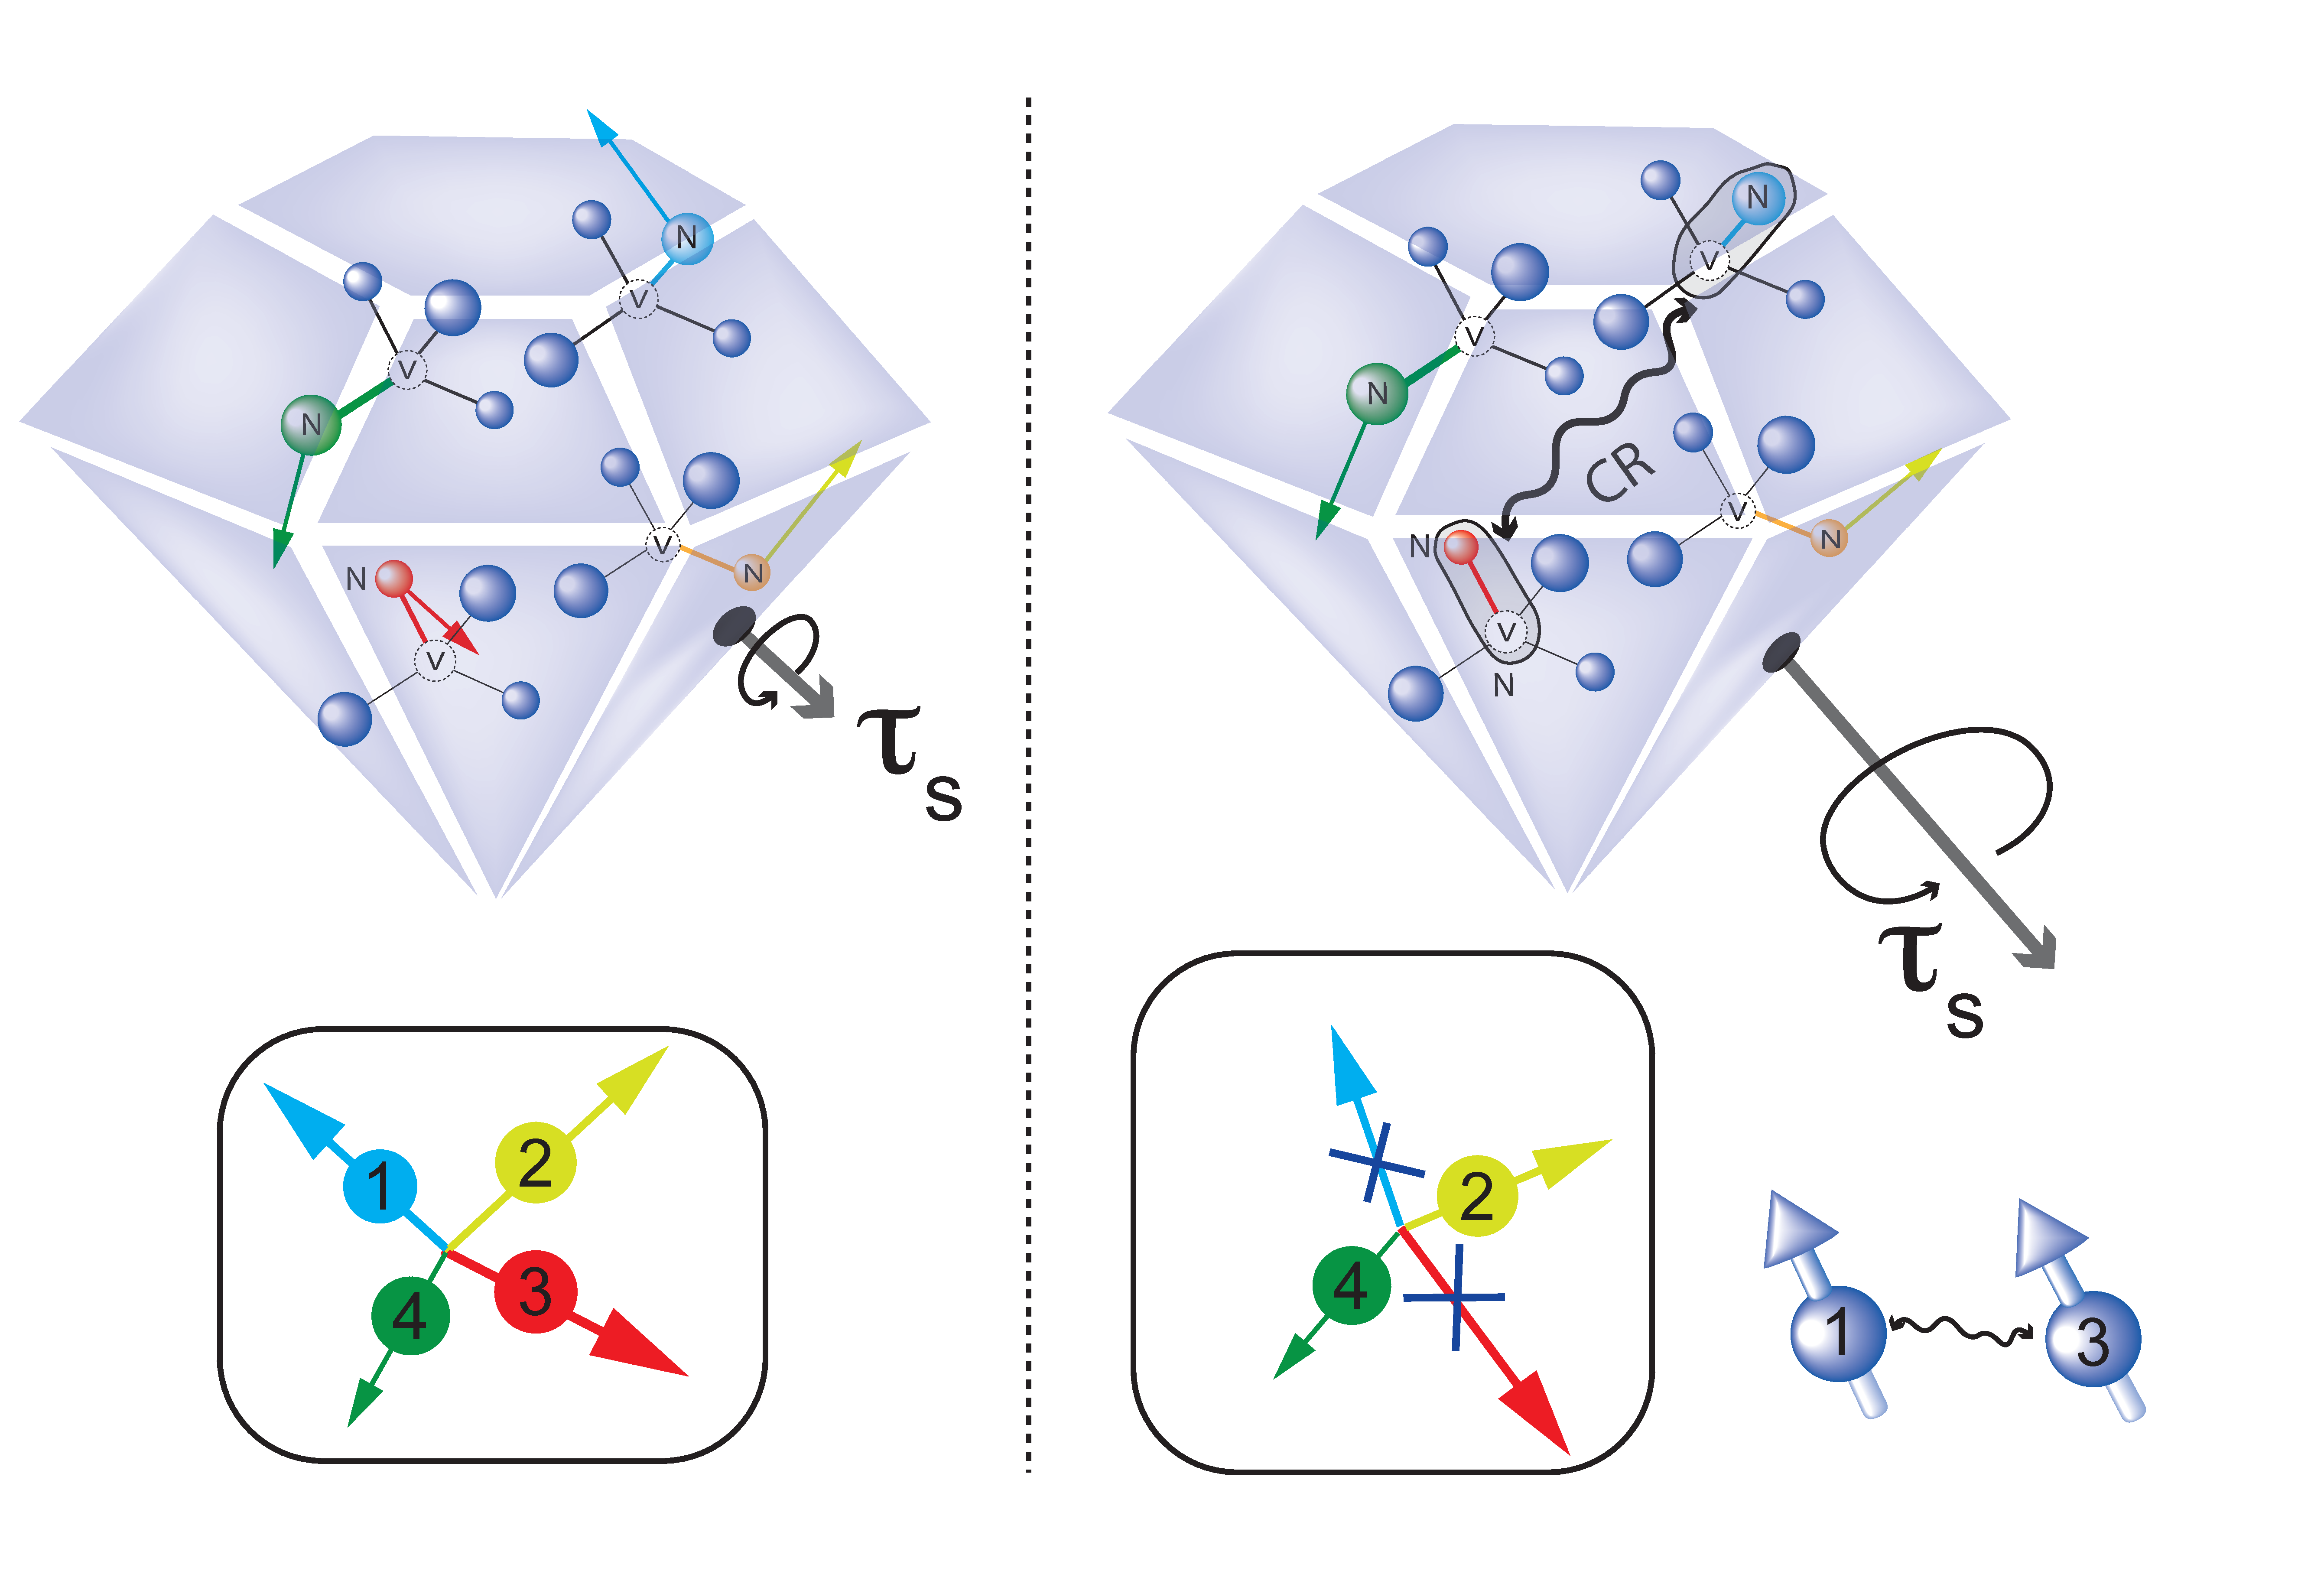
\includegraphics{dilutednv.pdf}}
  \caption{General principle of the resonant dipole-dipole induced mechanical rotation. The four possible directions of the nitrogen-vacancy centers in the diamond are shown in the left/right panels together with their spin-torque contributions (arrows of the corresponding colors). Left panel: the (quasi)-rotational invariance gives a small total spin torque $\tau_s$.
Right panel: A magnetic field (not shown) is tuned so that the spin class 1 and 3 point to the same direction. Cross-relaxation (CR) between these two classes of NV centers occurs, altering the rotational symmetry and increasing $\tau_s$. 
  }\label{principle}
\end{figure}

However, although the spin-mechanical coupling strength increases linearly with the number of atoms initially, new effects modify this scaling-law when the mean atom-atom distance is on the order of $\approx$ 10 nm. There, dipolar interactions amongst NV centers can become dominant, significantly enriching the physics at play. It has in fact been predicted that interaction amongst atoms can cooperatively enhance the coupling to the motion, akin to super-radiant processes \cite{Bachelard, PANAT}. 
Recent theory and experiments show that interactions between the optical dipoles NV centers enhances optical binding forces \cite{Venkatesh, Juan}. The interaction between the electronic spins of distant NV centers may also show similar spin-mechanical scaling. Further, the spin-interactions can be tuned resonantly amongst different NV orientations \cite{van_oort_cross-relaxation_1989}, offering prospects for studying the interplay between dipolar interactions and motional degrees of freedom in a controlled fashion. Increasing the density of NV centers also means that they can couple to other spins in the diamond \cite{armstrong_nvnv_2010, Alfasi, Epstein, Hall} and even transfer their polarization \cite{WangBajaj}.
When coupled to the angular degree of freedom, the latter effect would provide the unprecedented possibility to measure the exchange of spin angular momenta during cross-relaxation
%The laser-controlled spin-relaxation of NV centers enables a very high degree of control over the exchange of angular momenta between the spin and mechanical oscillators. 
%Coupling NV centers to impurities that cannot be optical polarized could then lead to interesting spectroscopic tools 
and enable controlling mechanical oscillators in the quantum regime \cite{Zangara}.  

%We then discuss how to cool a mechanical oscillator using CR. 

%When this occurs, the spin-torque is modified so that subsequently, the diamond rotates.
\begin{figure}[!ht]
  \centering \scalebox{0.08}{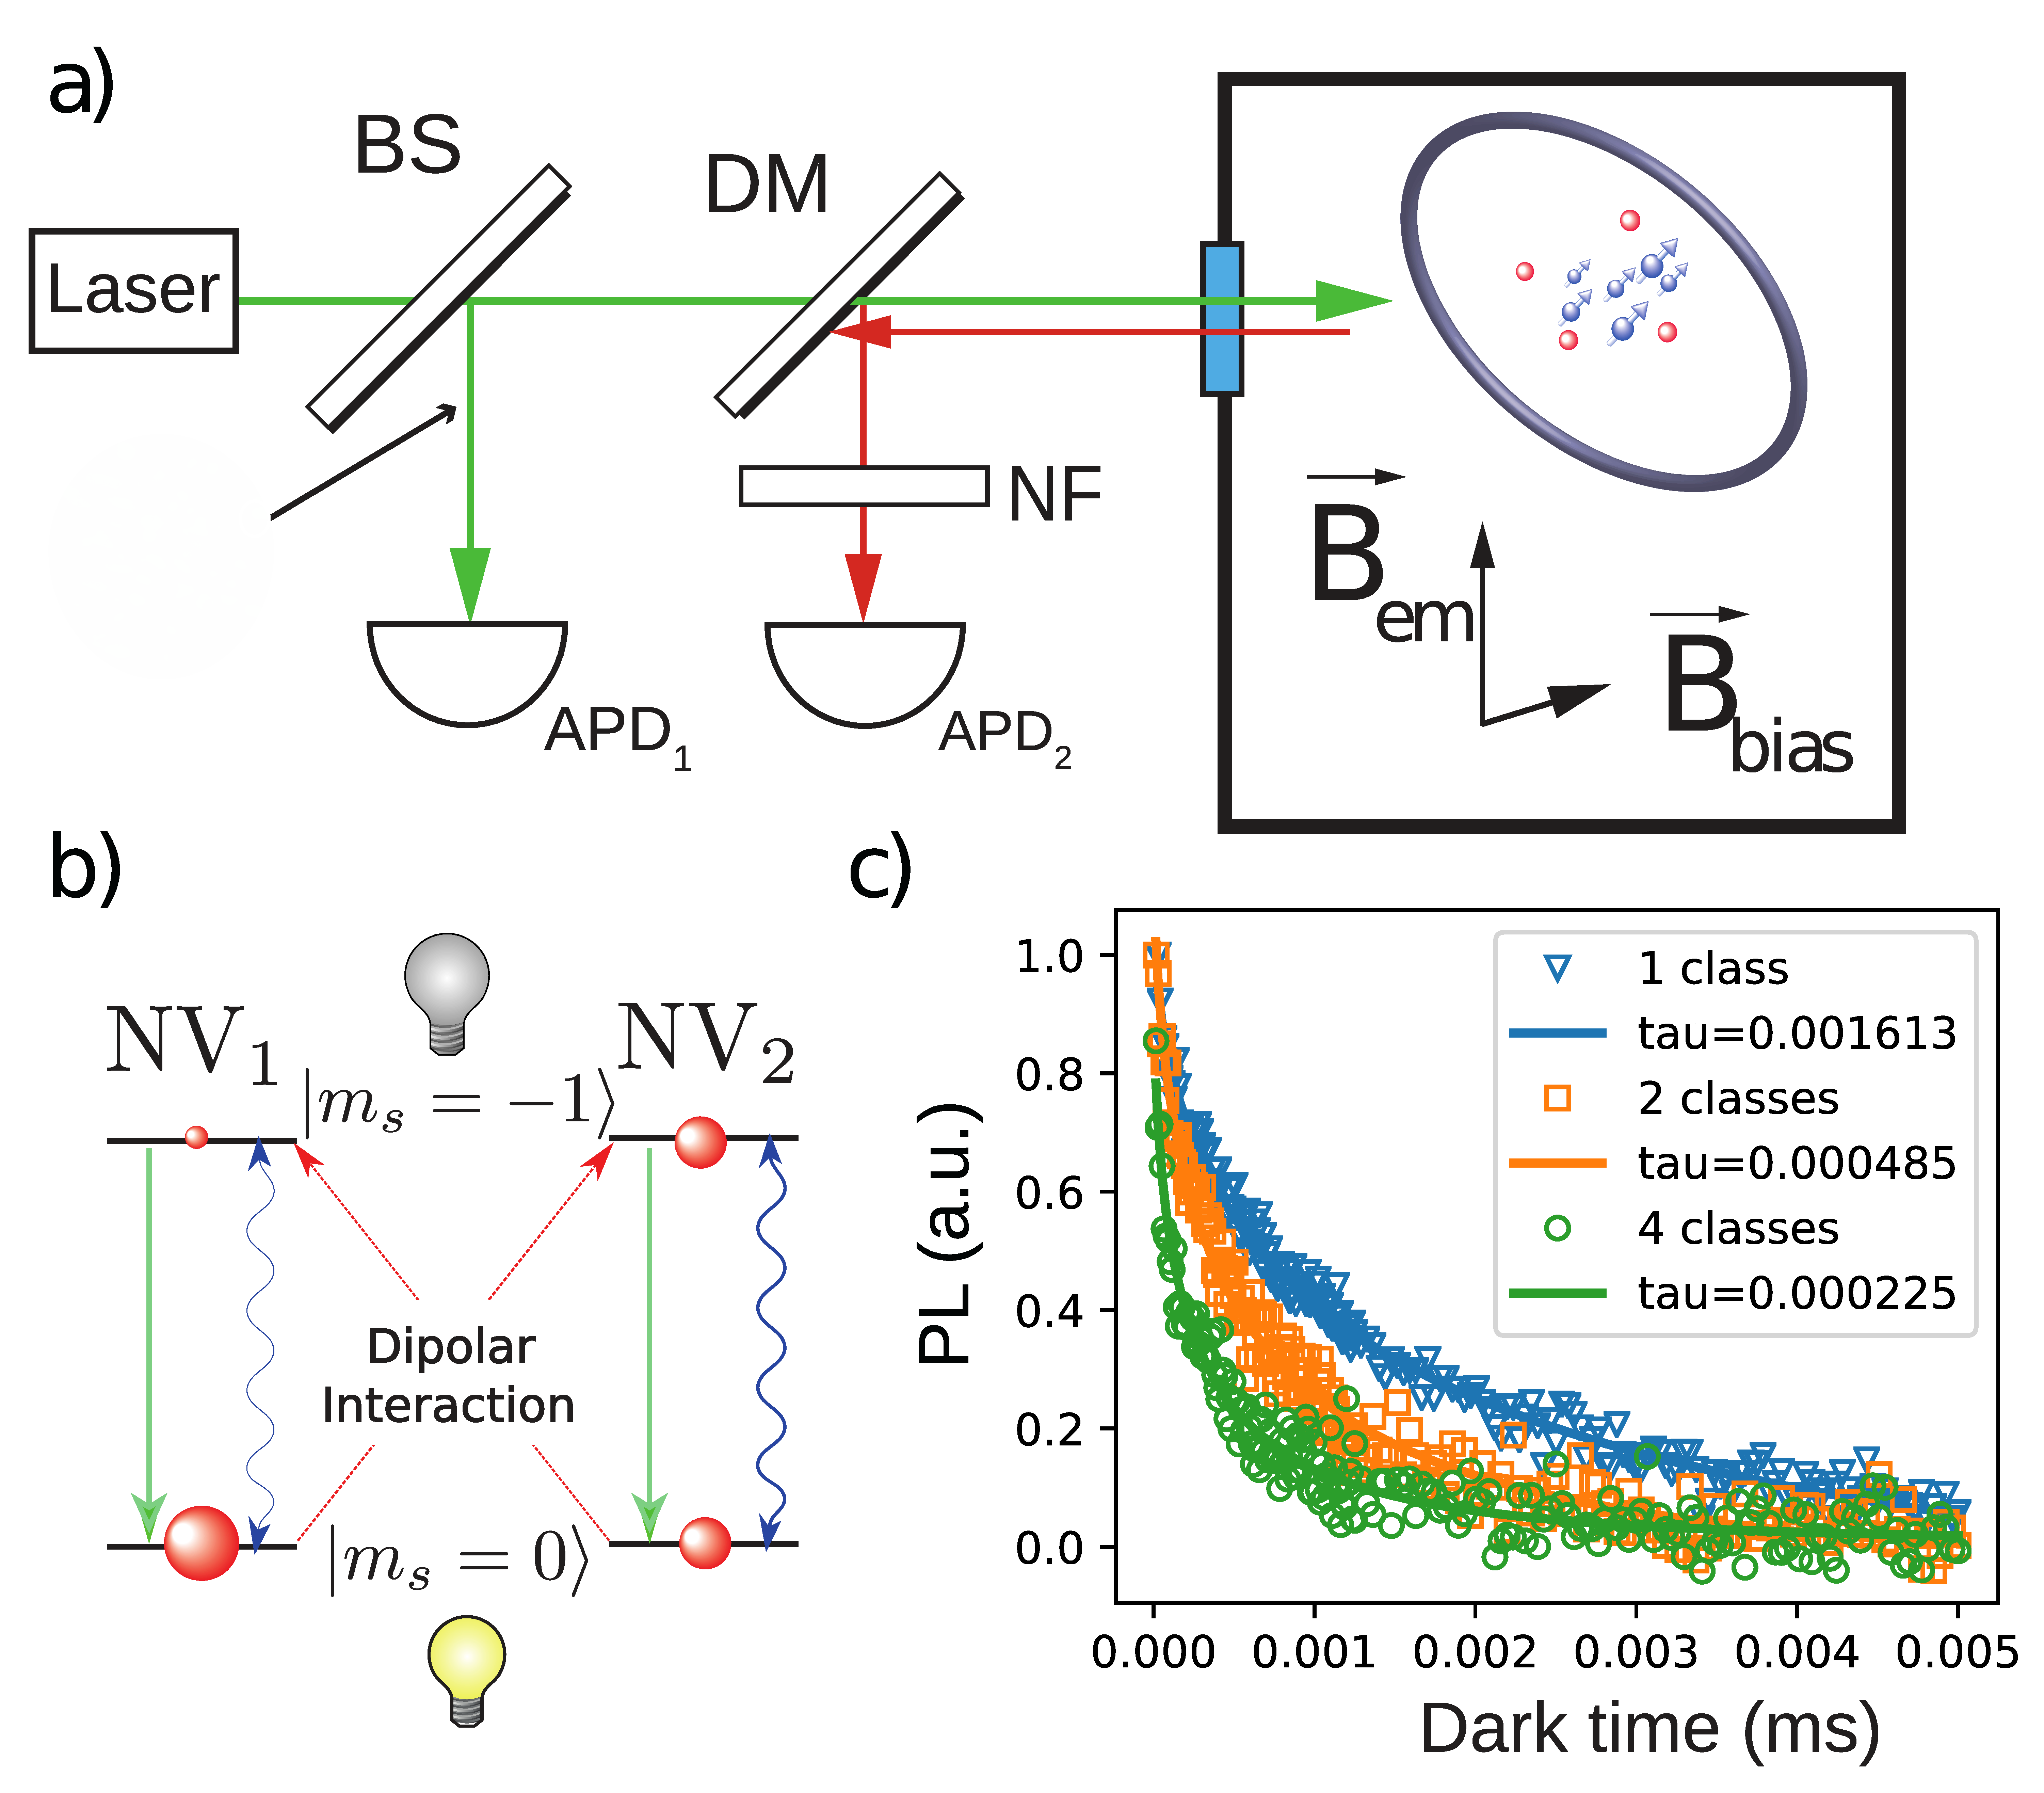
\includegraphics{setup.pdf}}
  \caption{Schematics of the experiment. A micro-diamond is levitating in a ring Paul trap enclosed in a vacuum chamber. A green laser is used both to polarize the NV centers in the levitating diamond and to detect the motion. Part of the speckle pattern formed in the image plane is sent onto APD$_1$ after passing through a beam splitter (BS). The photoluminescence from the NV centers is collected on APD$_2$ after filtering out the green laser light by a dichroic mirror (DM) and a notch filter (NF). a) Sketch showing the NV-NV depolarization process. Green arrows represent the optical pumping to the brighter $\ket{m_s=0}$ state. The two curvy blue arrows with different thicknesses represent short/long longitudinal relaxation of NV$_2$/NV$_1$. Red circles represent the population in each state and red dashed arrows represent the resonant dipole-dipole interaction between the two NV centers. c) Longitudinal relaxation from a single transition frequency. i) The class is not at resonance with any other classes : $T_1$=1.02 ms. ii) The class is at resonance with another class : $T_1$=0.28 ms. iii) The class is at resonance with the three other classes : $T_1$=0.15 ms.
  }\label{setup}
\end{figure}

Here, we employ resonant dipolar interactions between the spins of negatively charged nitrogen-vacancy centers to tune the orientation of a micro-mechanical oscillator. 
Specifically, we use NV centers inside a diamond that is levitating in a Paul trap and use resonant cross-relaxation between them to actuate
the spin-torque.
%We first present the results and conclude by discussing the potential applications behind our observations.
The key mechanism is depicted in Fig.~\ref{principle}. 
As can be seen in the left panel, NV centers can be found in four different orientations in the diamond crystalline structure. Due to quasi-rotational invariance of the problem, although each orientation could exert a significant torque to the diamond, the total spin-torque $\tau_s$ is very small.
%Our approach lies in the cross-relaxation (CR) that takes place when two spins with different orientations and polarization become resonant. 
%As depicted in Fig.~\ref{principle}-a), quasi-rotational invariance of the problem can make the sum of the spin torque of the four spin directions negligible. 
However by tuning an external magnetic field, resonant dipole-dipole interactions between the spin of NV centers of different orientations can be enhanced. 
When they become resonant, the polarization of the different orientations can then be exchanged in a process called cross-relaxation.
The right panel of Fig.~\ref{principle}, shows a cross-relaxation mechanism that partly removes the contribution from two classes of NV centers (labelled 1 and 3 in Fig.~\ref{principle}), which breaks the four-spin rotational invariance. The total spin torque $\tau_s$ can then be large enough to rotate the diamond.

%We first show that cross-relaxation can be effective in micro-diamonds that are heavily doped by NV centers.
%The NV center has two unpaired electrons in its ground state. In the triplet state, the dipolar interaction between them leads to a zero-field splitting $D=2.87$ GHz.
%The three spin states are labelled $| m_s={0}, {\pm 1}\rangle$.
%Due to an intersystem crossing in the optically excited state of the NV centers \cite{Doherty}, the state $m_s=\ket{0}$ is brighter than the state $m_s=\ket{\pm 1}$ upon green laser optical illumination \cite{Hopper}. 
%This provides a means to read out the Zeeman splitting by scanning a microwave tone around the resonance.
The diamonds that we use are in the form of a powder of particles that have a diameter of 15 $\mu$m. They are supplied by the company Adamas, which produces diamonds with a concentration of NV centers in the 3-4 ppm range. %The dipolar interactions may thus be effective since the average distance between the NV centers of about 10 nm. 
We load the micro-diamonds in a Paul trap that is similar to the one used in \cite{delordPRL} and depicted in Fig. \ref{setup}-a). One important feature of this system is the angular confinement provided by the trap, which offers the unique possibility to study the spin-induced torques.
Also, this geometry enables to apply a microwave signal directly on the trapping electrode, which provides an efficient means to excite the spins.
The photoluminescence from the NV centers is detected using standard confocal microscopy. We use about 100 $\mu$W of laser light at 532nm to polarize the NV centers. The laser is focused via a lens inside a vacuum chamber which has a numerical aperture of 0.5 and a working distance of 8mm. The focal point of the laser is kept few tens of micrometers away from the micro-diamond to mitigate the effect of radiation pressure and to enable laser excitation of the whole diamond \cite{delordPRL,delord2016}. 

\begin{figure}[!ht]
  \centering \scalebox{0.24}{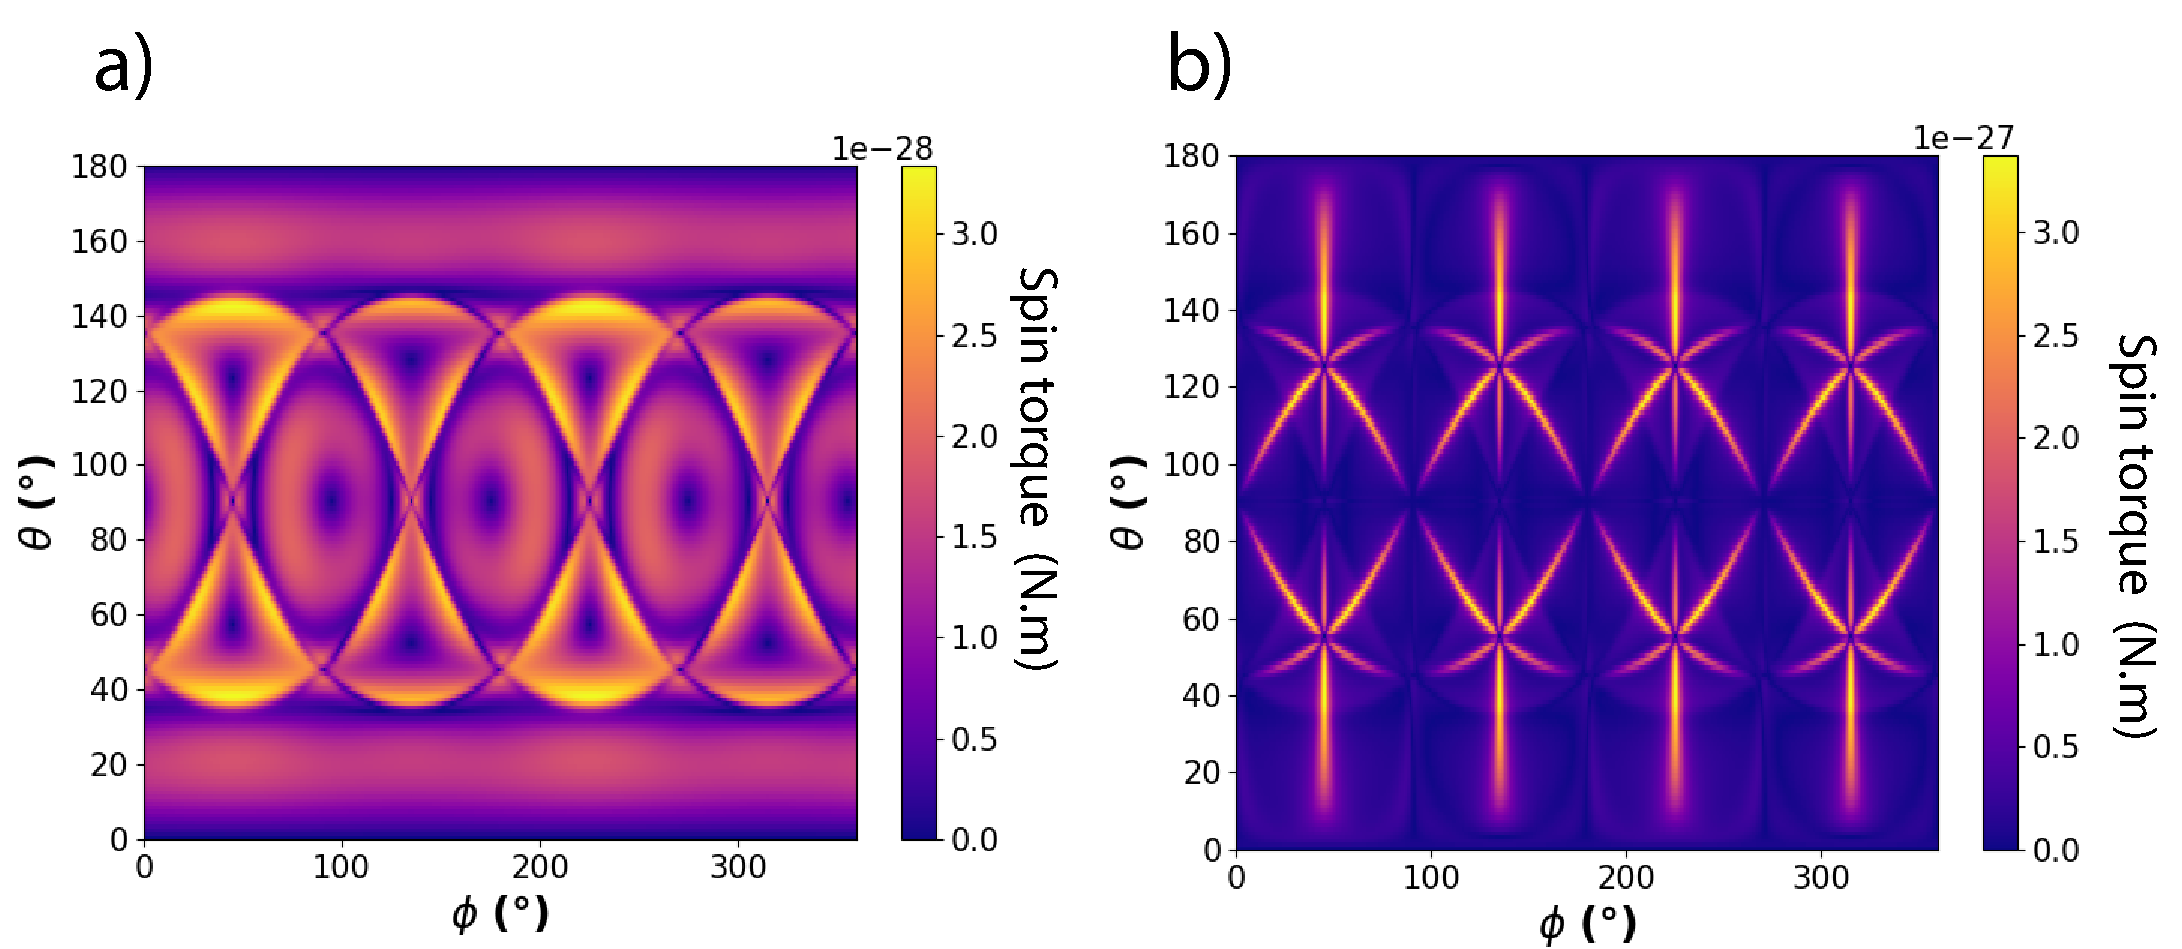
\includegraphics{map_torque_4_classe.pdf}}
  \caption{Numerical simulations of the spin-torques on a diamond containing one NV center per orientation as a function of $\theta$ and $\phi$, the polar and azimuthal angle with respect to the [100] direction. a) and b) show the torque with and without cross-relaxation between NV centers respectively.}
  \label{Numerics}
\end{figure}

%Let us first show that dipolar interactions are effective in our employed diamond micro-particles by studying cross-relaxation when they are simply attached to the trap. 
Fig.~\ref{setup}-b) depicts the dipolar interaction between two NV centers. In this example, the electronic spin of NV$_1$ is polarized in the ground state via the green laser, whereas NV$_2$ has a relaxation time $T_1$ that counteracts the influence of the optical polarization, reducing its total spin polarization. The spins will exchange magnetic quanta through flip-flop processes resulting in a depolarization of NV$_1$. At large enough NV densities, a few fast-decaying NV centers can then depolarize an ensemble of NV centers through dipolar interaction. This can reduce the average $T_1$ of the ensemble from the phonon-limited $T_1$ ($\approx$ ms) to a few hundreds of micro-seconds \cite{Jarmola} and lower the total photoluminescence. 
This effect has been observed by many groups \cite{van_oort_cross-relaxation_1989, armstrong_nvnv_2010, jarmola_longitudinal_2015, akhmedzhanov_microwave-free_2017, akhmedzhanov_magnetometry_2019, holliday_optical_1989, mrozek_longitudinal_2015, choi_depolarization_2017} in bulk materials. The origin of the fast-decaying NV centers was attributed to the presence of charge tunneling amongst closely packed NV centers \cite{choi_depolarization_2017}. The NV centers that undergo tunneling with other impurities (possibly with the substitutional nitrogen defect \cite{manson_nv_2018}) have a largely reduced longitudinal spin lifetime $T_1$.
%This process has recently revived interest because the sensitivity of magnetometers is ultimately limited by these interactions \cite{Zhou}. 
%In our spin-mechanics experiment, we use micro-diamond particules subjected to a green laser field and a magnetic field.
%To observe the dipolar effects in a levitating platform, we employ heavily doped micro-diamonds.

Such a process has not been presented with nano- or micro-particles in the literature to the best of our knowledge. Smaller diamond particles in fact tend to suffer from extra parasitic surface effects such as spin depolarization due to interaction with paramagnetic dangling bonds on the surface \cite{Tetienne}, or enhanced charge transfer between the NV$^0$ and NV$^-$ charge states \cite{Dhomkar} so it is essential to verify that it can be observed with micro-particles. 
We start by searching for CR using micro-diamonds that are physically attached to the trap, by employing a fixed bias magnetic field $||\bf B_{\rm bias}||\approx$100 G and by tuning another magnetic field $\bf B_{\rm em}$ at some angle with $\bf B_{\rm bias}$ using an electromagnet (see Fig.~\ref{setup}-b)). 

At specific magnetic field directions with respect to the crystalline axes, degeneracy between the spin of NV centers can be reached \cite{van_oort_cross-relaxation_1989}. %We check this systematically by searching for a reduction of the PL using APD$_2$ and using Opticall-Detected-Magnetic-Resonance (see SI) to correlated it with degeneracies. %We first characterize the depolarization of a diamond that is attached to trap ring to ensure that cross-relaxation can be observed in our samples.
%POUR LES SI 
%It is important to characterize this effect further when using smaller particles such micro-diamonds where surface effects can play a role. 
%where, to our knowledge, such cross-relaxations have not been observed. 
%Indeed, surface effects may start to play a role and change quantitatively.
In this case, the longitudinal decay time from NV centers should be reduced. To verify this, we measured the $T_1$ time by applying a green laser that polarizes the NV centers and measure the photoluminescence at a later time.
Such a measurement however turned out to be significantly impacted by recharging of NV centers in the dark \cite{choi_depolarization_2017, mrozek_longitudinal_2015, giri_selective_2019, giri_coupled_2018}.
In order to accurately measure the $T_1$ and remove the changing PL due to the recharging effects, we use the sequence presented in the SI, where a microwave pulse is applied or not prior to spin relaxation. The PL signals acquired in the two different measurements are then subtracted and shown for different degeneracy configurations in Figure \ref{setup}-c).
In the absence of degeneracy, we observe an exponentially decaying profile, from which we extract a $T_1=1.08$ ms, already shorter than the phonon limited lifetime in dilute bulk materials \cite{Tetienne}. This lifetime is even further reduced to 0.28 ms (resp. 0.15 ms) when two (resp. four) orientations are brought to resonance. This hints towards the role played by dipolar interactions, which are enhanced when classes of NV centers are resonant \cite{van_oort_cross-relaxation_1989, choi_depolarization_2017}. The effective density of NV being able to exchange spin quanta indeed increases, resulting in a stronger depolarization process.

%\begin{figure}[!ht]
%  \centering \scalebox{0.6}{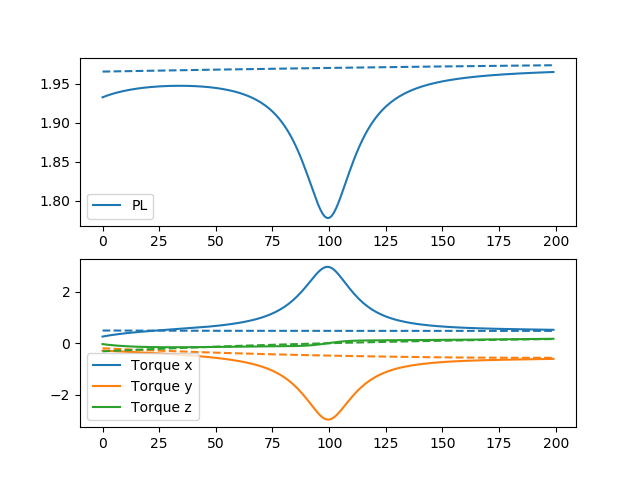
\includegraphics{cross_121_200G.png}}
%  \caption{Numerics : PL change in the presence of cross-relaxation (top) and spin-mechanical detection (below). 
%  }\label{CR_deposited}
%\end{figure}

The main goal our study is to search for the mechanical action of such dipolar induced relaxations with diamonds levitating in the Paul trap.
%Following the picture presented in Fig. 1, we will seek for changes in the diamond orientation at CR conditions. 
%For a given levitating particle, we can optimize, in real time, the signal coming from the angular displacement of the particle by selecting the most favorable region of the particle image. To do this, we monitor our optical signal while switching a microwave field tuned to one of the ESR transitions, at a frequency of 1 Hz.  Alignment is realized by maximizing the variation of the coupled light as the diamond rotates between two angular positions. 
One major basic ingredient is the spin-torque coming from the NV centers when they are polarized in the ground state. 
Let us consider first the dependence of the ground state energy of a single spin as a function of the angle between a magnetic field and the NV axis.
The Hamiltonian for one NV orientation with quantization axis $z$ in the particle frame reads 
\begin{equation}\hat{H}_{\rm NV}=\hbar D \hat{S}_z^2+ \hbar \gamma_e \bf B  \cdot \bf\hat S,
\end{equation}
where $\bf\hat S$ is the spin-vector, $D=(2\pi)2.87$ GHz the zero-field splitting and $\bf B$ is the external magnetic field.
Under the condition $\gamma ||\bm B|| \ll D$, and assuming an NV center and a magnetic field in an $(x,z)$ plane, $H_{B}=  \hbar \gamma_e {\bf B}  \cdot {\bf \hat S}=\hbar\gamma_e B  ( S_x \sin\theta + S_z \cos\theta)$ can be treated as a perturbation to the anisotropic part $\hbar D \hat{S}_z^2$ of the Hamiltonian. Here, $\theta$ is the angle between the magnetic field and the body-fixed NV center axis $z$.
The perturbed energy $\epsilon_g$ of the ground state due to the transverse B field $B_\perp=B \sin(\theta)$ is then
\begin{equation} \epsilon_g=\sum_{m_s=\pm 1}\frac{ |\bra{0} H_B \ket{\pm 1}|^2}{-\epsilon^0_{\pm 1}}=-\hbar\frac{(\gamma_e B_\perp)^2 }{D}
\end{equation}
\begin{figure*}[!ht]
  \centering \scalebox{0.45}{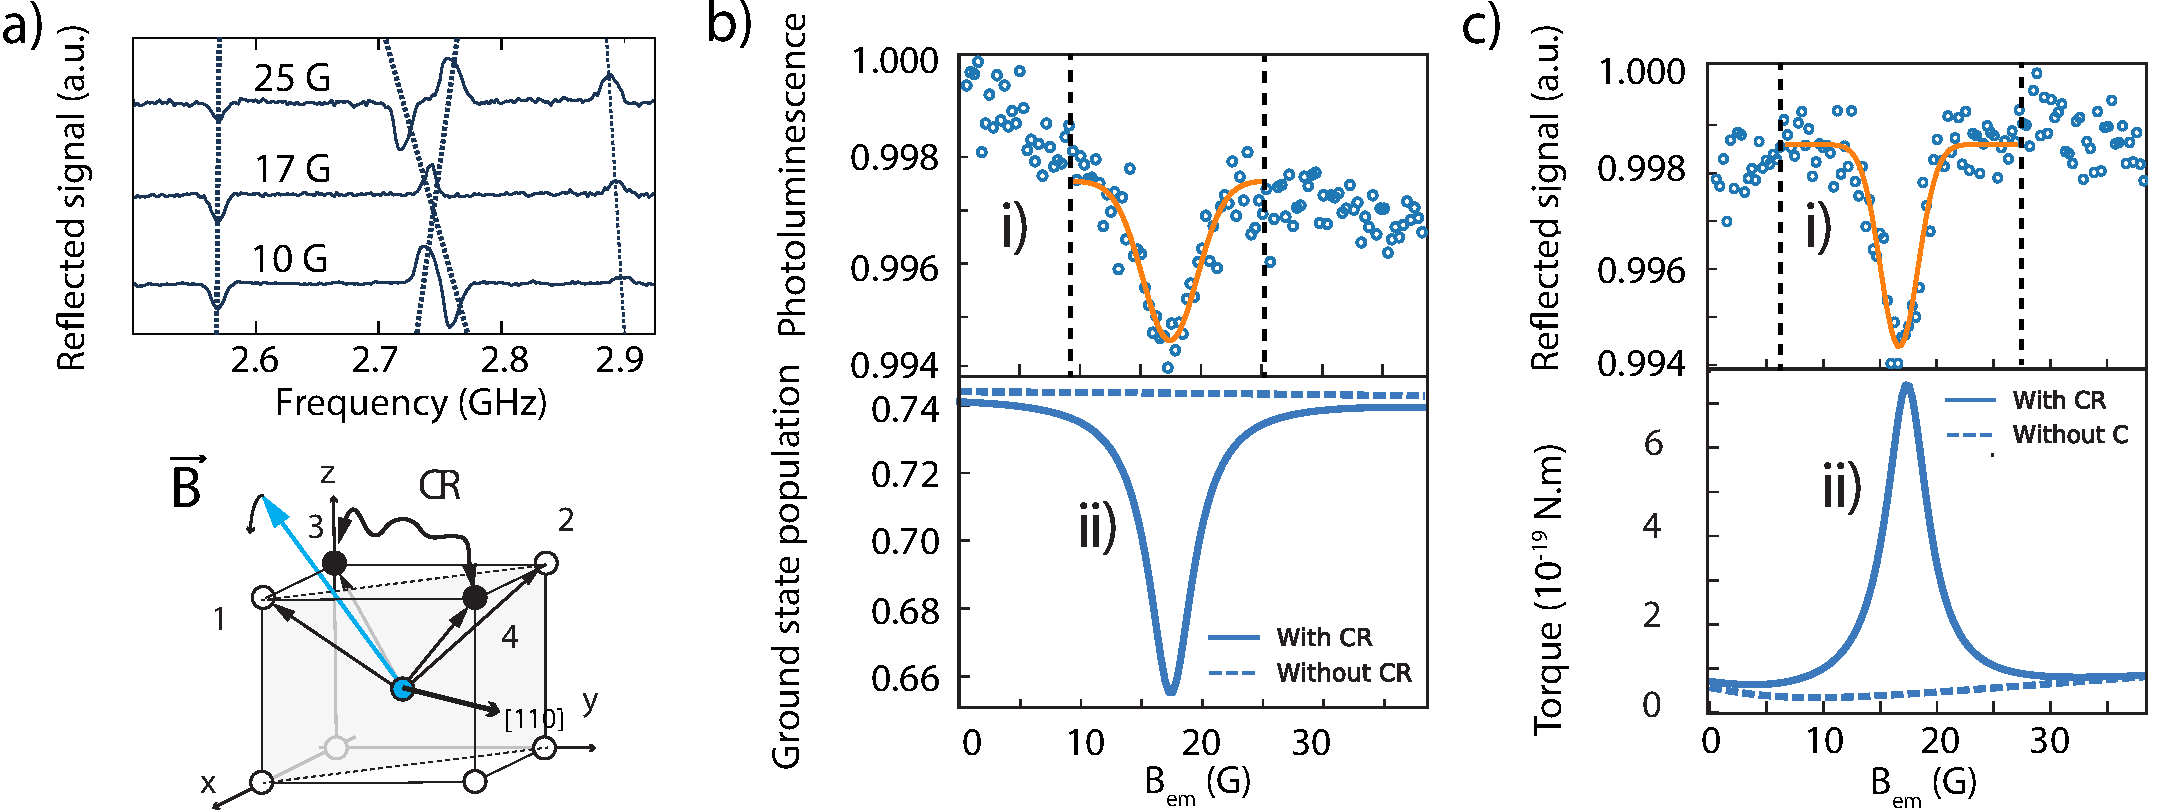
\includegraphics{CRmeca}}
  \caption{a) Top :  Signal reflected off the diamond surface as a function of microwave frequency for three different magnetic field values. Bottom : sketch showing the crossing of a crystal plane when the magnetic field angle is tuned.
b) PL detection as a function of B$_{\rm em}$ across a dipole-dipole resonance. i) experimental data with gaussian fit, ii) simulation of the population in $\ket{m_s=0}$ state, taking into account cross-relaxation (plain) or not (dashed).
c) Angular detection as a function of B$_{em}$ across a co-resonance. i) experimental data with gaussian fit, ii) simulation of the magnetic torque applied to the diamond, taking into account cross-relaxation (plain) or not (dashed).
  }
  \label{data}
\end{figure*}
A direct use of the Feynman-Hellman theorem can give the torque in the ground state. We find that 
\begin{equation}\tau_s=- \frac{\partial \epsilon_g}{\partial \theta}=\hbar  \frac{(\gamma_e B)^2}{D} \sin 2\theta.\label{Eq1}
\end{equation}
A proof of the applicability of this theorem is presented in the SI. 
At an angle $\theta=\pi/4$, where the torque is maximized and at a B field of 100 G, we find $\tau_s\approx 5\times 10^{-17}$ N.m. Using $10^9$ spins polarized in the ground state and taking a librational confinement frequency of the diamond in the Paul trap to be around $\omega_\theta/(2\pi)=1$ kHz, we obtain an angular displacement 
of $\tau/I\omega_\theta^2\approx$1 mrad, which can be measured with a high signal-to-noise ratio in our set-up \cite{DelordNat}.
%We checked numerically that at these magnetic field values and angle, the NV are still polarized mostly in the ground state. 
%Note that the torque is zero at $\theta=mod (\pi/2)$ where the eigenstates of $S_z$ are not mixed. 
%The Hamiltonian ground state is the eigenstate $| S=1,m_s=0\rangle$, which is is non magnetic. 

%Note also that the torque tends to zero if  tends to zero at any angle $\theta$. This is the case in the presence of strong spin-depolarisation, i.e. when $\hat\rho\rightarrow\frac{1}{3}\hat{I}$ (with $\hat{I}$ the identity operator).

As already hinted to in the explanations of Fig. 1, the contributions from the other NV classes must also be taken into account.
Fig. \ref{Numerics} presents the result of numerical calculations of the torque coming from the four classes of NV centers.   
Fig. \ref{Numerics}-a) shows the torque magnitude as a function of $\theta$ and $\phi$ without taking into account the cross-relaxations. The torque from each of the four classes appear clearly from the symmetry. Their different contributions however sum up to give a maximum torque of around $10^{-28}$ N.m, which is 20 times smaller than the torque that can be obtained for a single class due to the quasi-rotational invariance of the 4-NV classes. When two classes of NV center are resonant however, the induced cross-relaxation partly breaks this rotational invariance. 
Fig. \ref{Numerics}-b) shows the same plot, but including the effect of the cross-relaxation when classes of NV centers are degenerate (see SI).  
Here we use numbers that are deduced from our experimental observations of the CR induced change of the $T_1$.
One can see that a new pattern with larger spin-torque values is superimposed to the previous map. These larger values correspond to crossings of the crystal planes where NV degeneracies occur. 
At these coordinates, one recovers the torque estimation of Eq.~\ref{Eq1}, found for a single class, which would then imply a strong enough torque for overcoming the Paul trap confinement. 


%Fig. \ref{principle}-a) is a depiction of a levitating diamond containing NV centers that have four possible directions along the $\langle 111 \rangle$ axes. 
%In the presence of a magnetic field, each NV centers has a different magnetic field projection, which means a different torque. 
%Below, we show the sum of the ground state spin-torques $\tau_{NR}$, resulting from the four classes. 
%Fig. \ref{principle}-ii) shows the same situation, with a magnetic field that is tuned so that two NV classes are co-resonant. 
%When the re-polarization rate due to the green laser is smaller than the cross-relaxation rate, the magnetization coming from these two classes (indicated by a circle) tends to cancel. The population in the three NV eigenstates will indeed equilibrate, giving a smaller magnetization.
%The resulting torque is thus changed to $\tau_{R}$ and the diamond then turns about another angle.
%This is the essence of the proposed dipolar detection. 
%shows the total torque when 1-2-3-4 NV transitions are in the ground state. It is very small because the torque from 
%2-4 and 1-3 cancel each other. Looking at each pair 2-4 and 1-3 however, one can see that the torque is large (here 20 MHz for one spin).

To observe the effect of such resonant dipolar interactions experimentally, we use similar parameters and magnetic field arrangement than when the diamonds were not levitating. The diamond crystalline direction with respect to the magnetic field direction is characterized with greater precision than ODMR by recording the spin-torques given to the diamond when a microwave drives the spin to the $m_s=-1$ state. 
The angle detection is performed by collecting the back-reflected green light from the diamond interface (see Fig. 2), separated from the excitation light using a beam splitter. 
Fig. \ref{data}-a) shows spin-mechanical detection of spin-resonances for three different $\bf B_{\rm em}$ amplitudes. 
At 10 and 25 G, one can observe 4 peaks in the spectrum that demonstrate spin induced torque on the diamond from the 4 classes of NVs.
At 17 G however, two classes merge at 2.75 GHz. This is where we expect to observe CR. 
%Note that perfect degeneracy would still make the diamond rotate when performing microwave scans since the microwave polarization is not the same for the two classes, and thus does not drive equally the two spin transitions. 

Analysis (SI) suggest that here, since we observe a single degeneracy, the magnetic field crosses a plane that is perpendicular to the $(110)$ direction as shown in Fig. \ref{data}-a).
Fig. \ref{data}-b) shows the photoluminescence as a function of $\bf B_{\rm em}$ both experimentally (trace i) and numerically (trace ii).
As expected, the PL decreases across the degeneracies at around the same magnetic field value, as a consequence of the CR-induced reduction of the $T_1$ time.
Fig. \ref{data}-c), trace i) is a measurement of the diamond angular position acquired simultaneously to the PL. Trace ii) is the corresponding calculation.   
A pronounced variation of the reflected signal is also observed, demonstrating here the close correspondence between degeneracy and diamond rotation and letting us conclude that we are observing a significant change in the spin-torque as the dipolar interactions between the spins increase. Note that as opposed to the PL detection, the signal coming from the particle surface can increase or decrease depending on how the speckle is aligned to the fiber. This explains the differing shapes of the signals in the experiments and the simulations. 
Fitting this curve by a Gaussian, we deduce a width that is similar to the PL width (1.3G and 1.7G respectively). This gives a width of X MHz ? comparable to ???
Similar experiments were realized on different particles under different degeneracies and similar effects were observed.
In the SI, we show similar results taken under different bias magnetic fields and under a two-fold degeneracy. 
%Note that the present effect cannot be attributed to a change in the angular momentum, as in the Einstein de Haas effect. 
%The latter would manifest itself for much smaller particles sizes. Further, the rotation would occur dynamically and not manifest itself as a static torque as is the case in the present experiment. 

Let us conclude by mentioning the applications offered by our work. 
The observed resonant dipole-dipole induced mechanical rotation can be employed to control the temperature and stiffness of mechanical oscillators. 
For this, a delayed dynamical back-action from the diamond magnetization to the mechanical oscillator is required \cite{Aspelmeyer} in order to increase the imaginary part of the spin-mechanical susceptibility \cite{DelordNat}.
At a magnetic field value corresponding to a negative detuning from the CR feature, the NV fluctuator will partly depolarize the spins and let the two other transitions apply a torque until the spins re-polarize back, thus produces a potentially efficient cooling cycle under vacuum.  % In essence, this would be the analogue of the spin-cooling shown in \cite{DelordNat}, but without using microwave and using dipolar-coupled spins. 

Conversely, our demonstration can be viewed as a novel spectroscopic technic to mechanically sense dipolar interactions between NV centers and spins that cannot be polarized optically.  Using the above cross-relaxation effect, one could use a magnetic field that is oriented along the [111] direction and detect paramagnetic species that do not have 
a strong anisotropy using a magnetic field gradient.  This opens a path towards the investigation of angular momentum conservation during the relaxation processes \cite{Zangara}.
%ODMR and EPR detect energies shifts but not angular momenta.  It would be beneficial to detect the dipolar interaction using the motion of the body itself in order to gain knowledge about angular momentum exchange as proposed in .
%The dipolar interaction can readily be detected indirectly using the motion of the object itself or via the Zeeman shift or motion of close paramagnetic or ferro-magnetic objects in the presence of a magnetic field. 

Last, and more prospectively, one could consider this work to be a kind of bottom-up approach for magnetism, where both the interaction and the relaxation can be tuned in order to reproduce the behaviors of a magnet. (may also form a testbed for nano-magnetism).
The detailed microscopic origin of magnetism depends a lot on the material and the relaxation mechanism is not controlled and is very short, making measurements of the  Gilbert-damping a complicated task.
%The microscopic origin of the angular momentum exchange is also not well-understood. 
Our work may thus open a path towards using NV centers to probe microscopic effects that take place in nano-scale magnetism. 

%To conclude, we demonstrate dipole-dipole induced rotation of a levitating diamond containing nitrogen-vacancy (NV) centers. 
%Our demonstration opens a path towards the use of mechanical oscillators to detect paramagnetic defects that lack optical transitions, to investigation of angular momentum conservation in spin relaxation processes and to novel means of cooling the motion of mechanical oscillators.

\section*{acknowledgements}
GH acknowledges SIRTEQ for funding.

\bibliography{trap}



\end{document}